\documentclass[12pt]{article}

\usepackage[utf8]{inputenc}

% \usepackage[papersize={2000mm,800mm},width=2000mm,height=800mm,centering]{geometry}
% \usepackage[papersize={1000mm,400mm},width=1000mm,height=400mm,centering]{geometry}
\usepackage[papersize={500mm,200mm},width=500mm,height=200mm,centering]{geometry}

% \usepackage{mathptmx}
%\usepackage{palatino}

%\usepackage{chancery}
%\usepackage{antiqua}
%\usepackage{aboensis}
\usepackage{gfsartemisia-euler}
\usepackage[T1]{fontenc}

% \usepackage{fontspec}
% \setmainfont{QTChanceryType}

\usepackage{graphicx}
\usepackage[table]{xcolor}
\usepackage{tikz}
\usetikzlibrary{decorations.text}
\usepackage[hidelinks]{hyperref}

\pagestyle{empty}

\newcommand{\logo}{\makebox[56mm][c]{\rule{0mm}{66mm}\raisebox{12mm}{\includegraphics[width=48mm]{logo/aldc-4couleurs-3.pdf}}}}

%\pagecolor{yellow!5}

\usepackage{fontspec}


\begin{document}
%\sffamily
%\bfseries
%\color{yellow!20}
\parindent=0mm

\fontspec{QTOKCorral-Ext}
\fontsize{64pt}{64pt}
\selectfont

\unitlength=0.5mm
\begin{picture}(0,0)
%%%%%%%%%%%%%% FOND ET LOGOS
% \put(240,-550){\includegraphics[height=300mm]{levis3.jpg}}
\put(100,-425){\includegraphics[height=250mm]{images/good/pJKzu5Oj.jpeg}}
% \put(0,-400){\includegraphics[height=205mm]{panorama1.jpg}}
% \put(0,-400){\includegraphics[height=205mm]{panorama2.jpg}}
%\put(-5,-400){\includegraphics[height=405mm]{images/Fond-bois-tres-clair-small.jpg}}
\put(-5,-400){\includegraphics[height=205mm]{../images/Fond-bois.jpg}}
\put(5,-375){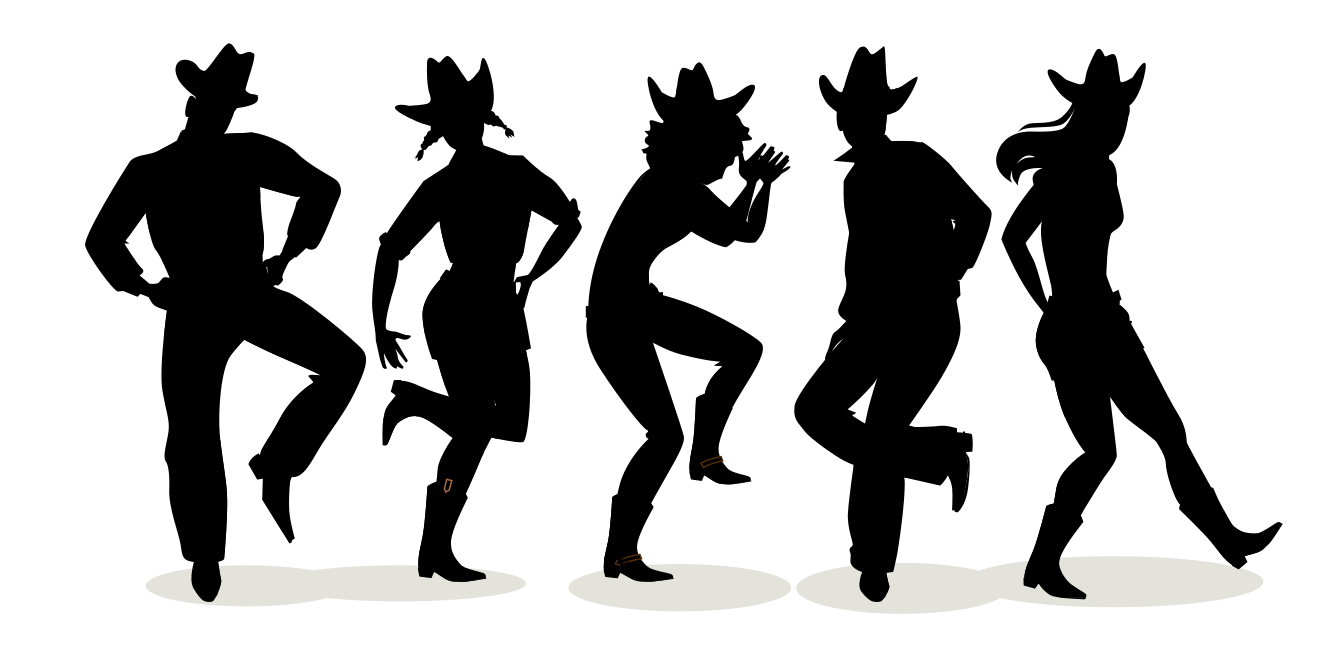
\includegraphics[width=120mm]{../images/groupededanseenligne-ombre.pdf}}
\put(10,-220){\href{https://alevisdanse.github.io}{\includegraphics[height=100mm]{../static/images/logo-aldc-sans-contour.pdf}}}
\put(850,-120){\href{https://alevisdanse.github.io}{\includegraphics[height=60mm]{../static/images/logo-aldc-contour-noir.pdf}}}
%\put(180,-350){\href{https://alevisdanse.github.io}{\includegraphics[height=80mm]{../static/images/logo-aldc-sans-contour.pdf}}}
\put(280,-350){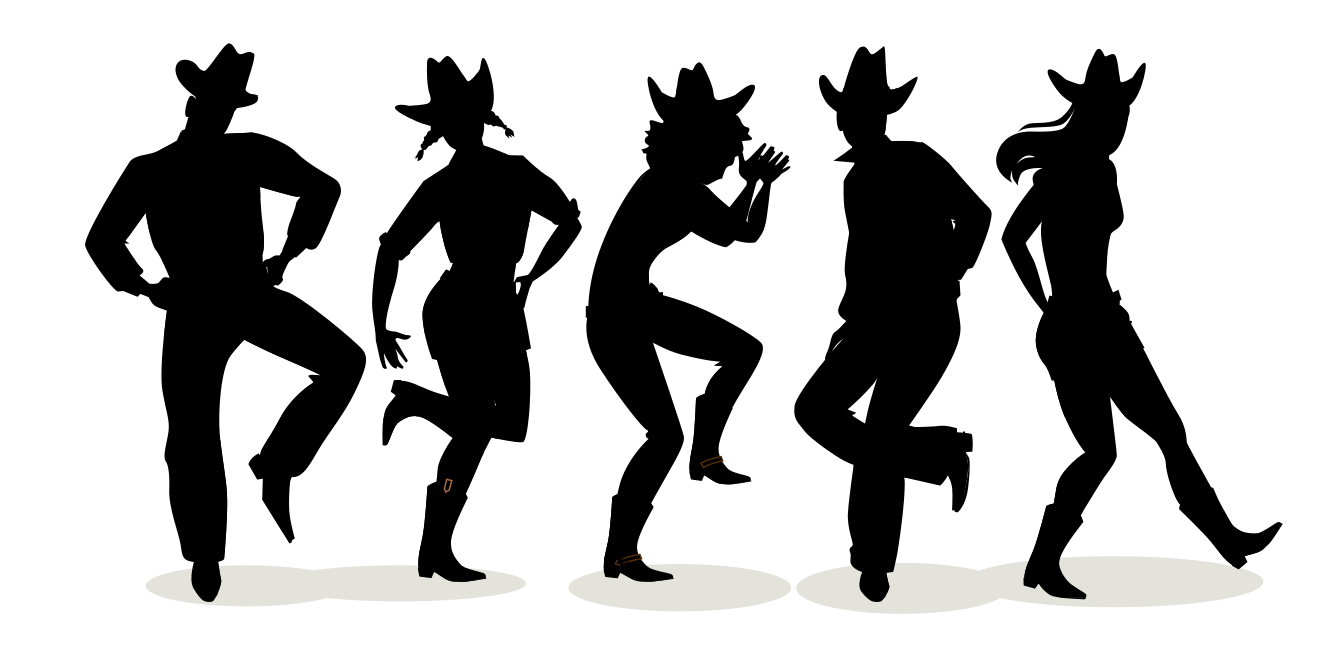
\includegraphics[width=300mm]{../images/groupededanseenligne-ombre.png}}
%\put(420,-360){\color{red!50}(C'est juste un exemple de texte !)}
%\put(417,-357){(C'est juste un exemple de texte !)}
% \put(250,-220){\begin{tikzpicture}
% \node (a) at (0,0){};
% \node (b) at (22,0){};
% \node (aa) at (0.15,-0.15){};
% \node (bb) at (22.15,-0.15){};
% \draw[draw=none, postaction={decorate,decoration={text along path,text align=center,text color=yellow!20,text={The Very Best of Line Dancing}}}] (aa) to [bend right=-20]  (bb);
% \draw[draw=none, postaction={decorate,decoration={text along path,text align=center,text={The Very Best of Line Dancing}}}] (a) to [bend right=-20]  (b);
% \end{tikzpicture}}
% \put(280,-400){\begin{tikzpicture}
% \node (a) at (0,0){};
% \node (b) at (25,0){};
% \node (aa) at (0.15,-0.15){};
% \node (bb) at (25.15,-0.15){};
% \draw[draw=none, postaction={decorate,decoration={text along path,text align=center,text color=blue!20,text={in the Famous High Valley of Yvette}}}] (aa) to [out=20,in=-140]  (bb);
% \draw[draw=none, postaction={decorate,decoration={text along path,text align=center,text={in the Famous High Valley of Yvette}}}] (a) to [out=20,in=-140]  (b);
% \end{tikzpicture}}
\put(250,-250){\begin{tikzpicture}
\node (a) at (0,0){};
\node (b) at (34,0){};
\node (aa) at (0.15,-0.15){};
\node (bb) at (34.15,-0.15){};
\draw[draw=none, postaction={decorate,decoration={text along path,text align=center,text color=orange!50,text={Oui à Lé-, vis-Saint-Nom, on y danse, on y danse}}}] (aa) to [out=20, in=-160]  (bb);
\draw[draw=none, postaction={decorate,decoration={text along path,text align=center,text={Oui à Lé-, vis-Saint-Nom, on y danse, on y danse}}}] (a) to [out=20, in=-160]  (b);
\end{tikzpicture}}
\put(260,-400){\begin{tikzpicture}
\node (a) at (0,0){};
\node (b) at (36,0){};
\node (aa) at (0.15,-0.15){};
\node (bb) at (36.15,-0.15){};
\draw[draw=none, postaction={decorate,decoration={text along path,text align=center,text color=orange!50,text={Oui à Lé-, vis-Saint-Nom, on y danse, tous en ligne}}}] (aa) to [out=-30,in=180]  (bb);
\draw[draw=none, postaction={decorate,decoration={text along path,text align=center,text={Oui à Lé-, vis-Saint-Nom, on y danse, tous en ligne}}}] (a) to [out=-30,in=180]  (b);
\end{tikzpicture}}
\end{picture}


\end{document}


%%% Local Variables:
%%% TeX-engine: luatex
%%% End: